\chapter{Summary and future developments}
\subsection*{Summary}
In this work, we have studied two-layers fully-connected neural networks in the teacher-student setting.
We derived deterministic equations for the evolution of the order parameters in the case of the activation function \(\sigma(x)=x^2\),
and pointed out how this may fall into a famous model studied: phase retrieval.
We explored many possible initial conditions and analyzed the symmetries they may introduce.
We arrived at writing an early formula for learning time in the specific case of phase retrieval, noting,
however, that it is not too informative since it is influenced by the norm of the chosen initial conditions.

We then introduced the spherical constraint in order to directly analyze the phases of the learning of our interest.
We derived the differential equations describing the dynamics in this situation and set initial conditions based on what we comprehended previously.
We were able to derive a complete description of phase retrieval dynamics that, among other things,
allowed us to write an explicit formula for an exit time; we verified that it was in agreement with when previously known from the literature.
We then repeated the analysis first for generalized phase retrieval, then for a generic neural network, obtaining discrete results.
We have shown that from learning times it is possible to give an estimate of the gain that is obtained in enlarging the first layer of the network.
By exploring different regimes, we realized that the ratios between the exit time of an overparametized network and one that is not, are finite:
therefore, there is a maximum speed-up that can be achieved, at least at the stage of learning under consideration.

In the last part, we tried to add a corrective term to the equations used for the previous analysis. The added correction is nondeterministic and transforms the equations into stochastic processes, which we approximated through Brownian motions.
For simplicity, we limited ourselves to the phase retrieval analysis. 
First, we applied the corrections to the unconstrained case and showed that they worked and were in agreement with a work that came out in conjunction with our study.
As in the deterministic case, however, we could not derive a formula for exit time. We then moved on to the constrained case on the sphere, where the first difficulty was figuring out how to write the stochastic process.
Through the Itô calculus, we obtained a correct description of the dynamics and,
through the necessary approximations, derived a formula for the exit time.
Comparing the results with those obtained previously from the differential equations,
we found that the corrections allow for a more accurate estimate of the learning time,
leaving several possibilities for future analysis with this tool. 

\subsection*{Future Developments}
There are many directions that can be explored now.
The natural next step to the last part of the results presented in this paper is to derive a description with stochastic processes for the generalized phase retrieval and the generic network as well.
Having more accurate formulas for the output times would allow us to make more precise statements about the gain benefited by overparameterization.
This involves analyzing several stochastic processes, but it should be feasible and has not been analyzed here simply for lack of time.

Another question that arises is whether the analysis done now can be repeated for the specialization phase of learning. Referring to Figure~\ref{fig:pictorial-symmetric-learning2}, we studied the exit time for the blue curve, but not the exit time for the green. 
In the plots of the risk we represented we could see only one drop because with the activation function we chose the two transitions occurred so close together that the plateau between the two is not visible, (besides that this phase is really only present when \(k>1\)). 
One could look for initial conditions that are already in the blue plateau, so as to study only the specialization. Another alternative is to choose a different activation function, where the separation of the two phases is sharper. 
This choice would be beneficial since it would also allow us to use more realistic activation functions such as ReLU or erf.
If the previous goal were to be achieved, one could then consider making the networks deeper and see how the output times relate as a function of the width of the various layers. This is an ambitious task, but a stepwise analysis could lead us to some good results.
\begin{figure}
  \centering
  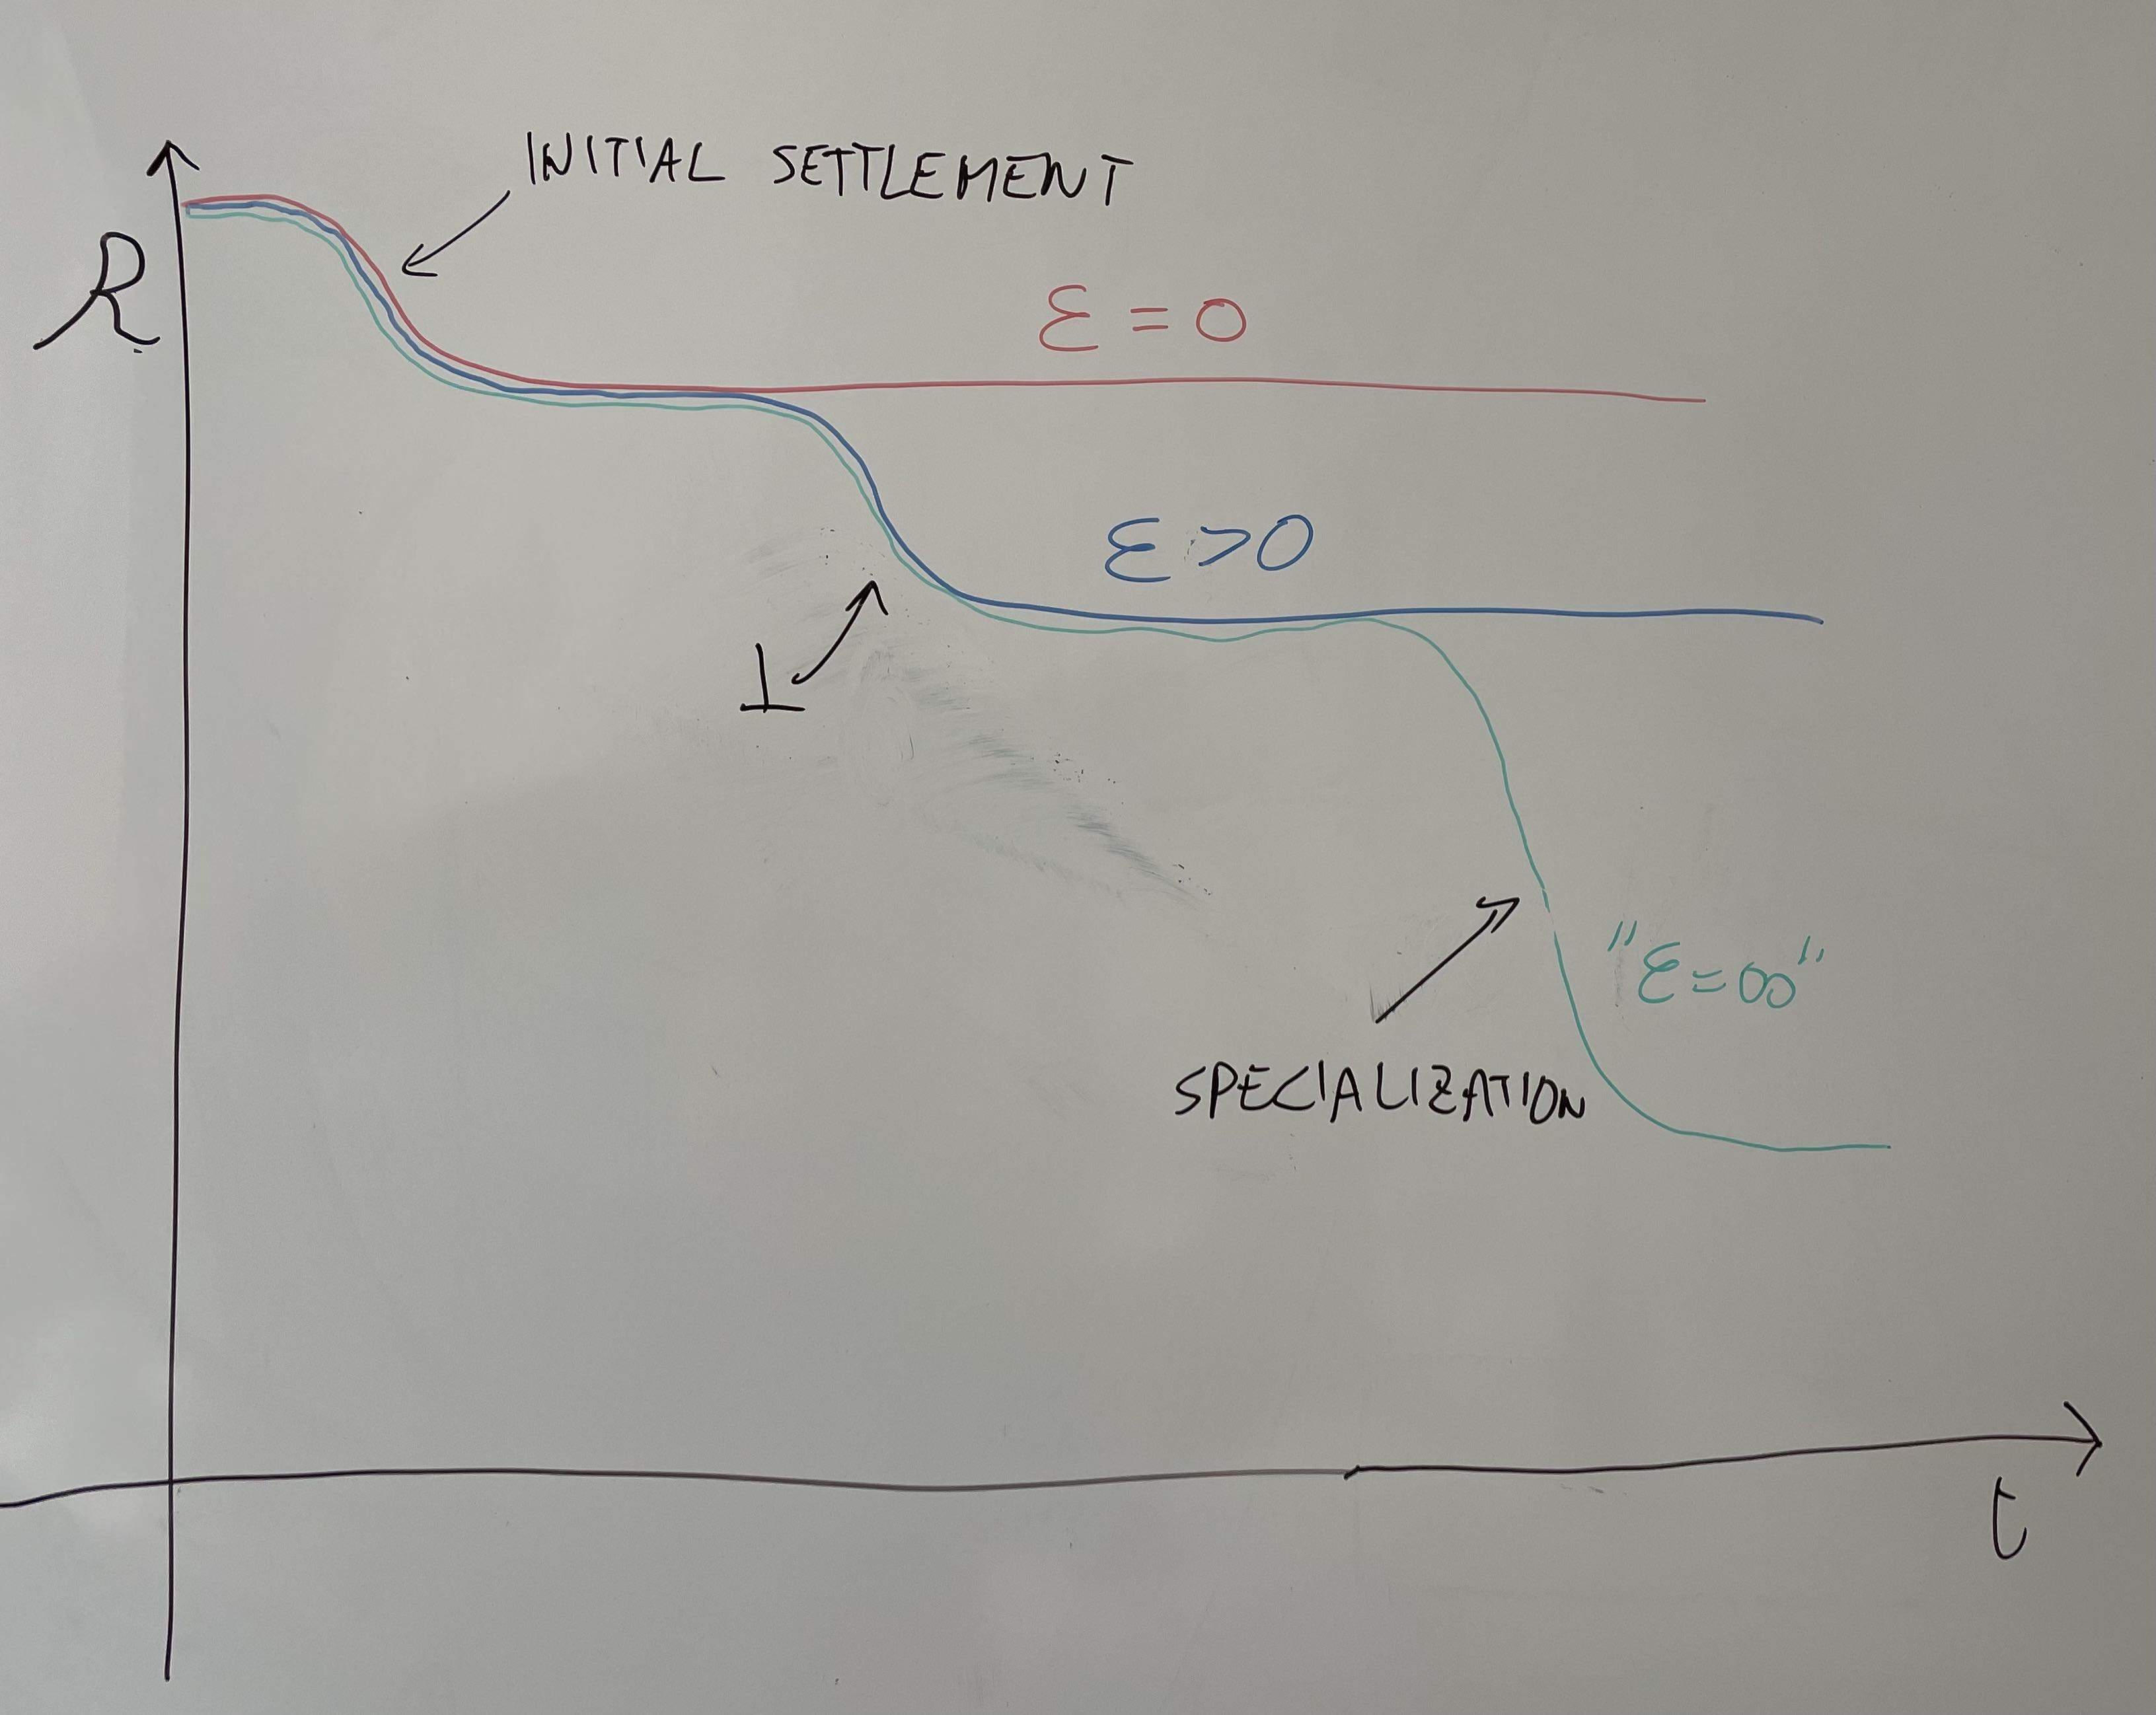
\includegraphics[width=.7\textwidth]{figures/symmetric-ic-expected-plateaus.jpg}
  \caption{
    pictorial representation of the different phases of learning for symmetric initial conditions.
  }
  \label{fig:pictorial-symmetric-learning2}
\end{figure}

Changing perspective, one could study the connections of what we have done with a line of work analyzing the mean-field limit on strongly overparametrized networks \cite{mei2018mean, chizat2018global,rotskoff2018trainability, sirignano2020mean}.
In these papers, they keep fixed the input dimension while they take the limit \(p\to+\infty\);
they find some PDEs on weights probability density that can be used to infer properties of the learning dynamic.
We would therefore like to investigate whether in this different limitation we reach the same conclusions as we do and possibly develop a theory that encapsulates both,
thus arriving at a complete understanding of neural network behavior.

In conclusion, there is still a lot of work to be done within this setting; however, this thesis has collected some results that can be expanded and generalized to arrive at a more comprehensive view of two-layer neural networks. We hope that this work can be a valuable starting point for several future investigations.